\documentclass{article}
\usepackage{tikz}
\usetikzlibrary{shapes.geometric, arrows, positioning, calc}

\begin{document}
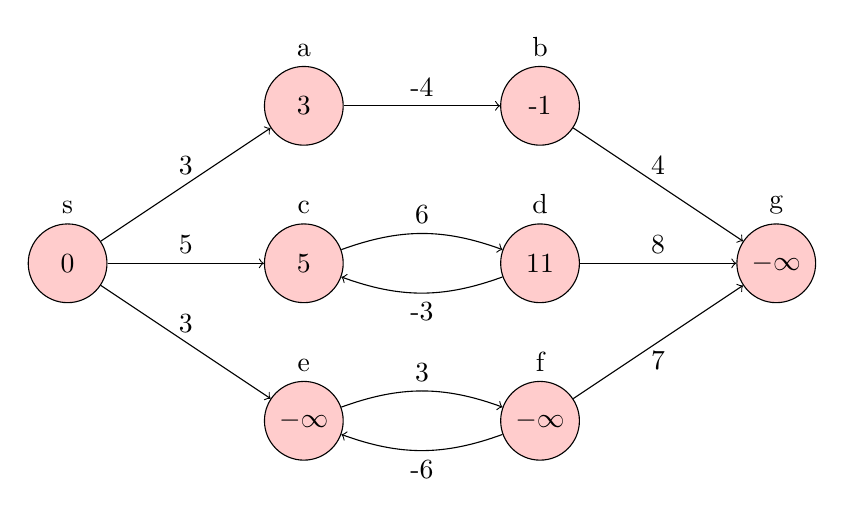
\begin{tikzpicture}
%nodes
\node[circle, draw, fill=red!20,minimum size=1cm,label=above:s] (a) at (0, 0) {0};
\node[circle, draw, fill=red!20,minimum size=1cm,label=above:c] (b) at (3, 0) {5};
\node[circle, draw, fill=red!20,minimum size=1cm,label=above:d] (c) at (6, 0) {11};
\node[circle, draw, fill=red!20,minimum size=1cm,label=above:g] (d) at (9, 0) {$-\infty$};
\node[circle, draw, fill=red!20,minimum size=1cm,label=above:a] (e) at (3, 2) {3};
\node[circle, draw, fill=red!20,minimum size=1cm,label=above:b] (f) at (6, 2) {-1};
\node[circle, draw, fill=red!20,minimum size=1cm,label=above:e] (g) at (3, -2) {$-\infty$};
\node[circle, draw, fill=red!20,minimum size=1cm,label=above:f] (h) at (6, -2) {$-\infty$};

%connections
\draw[->](a) to node[above]{5}(b);
\draw[->,bend left=20](b)to node[above]{6}(c);
\draw[->,bend left=20](c)to node[below]{-3}(b);
\draw[->](c) to node[above]{8}(d);
\draw[->](a) to node[above]{3}(e);
\draw[->](e) to node[above]{-4}(f);
\draw[->](f) to node[above]{4}(d);
\draw[->](a) to node[above]{3}(g);
\draw[->,bend left=20](g)to node[above]{3}(h);
\draw[->,bend left=20](h)to node[below]{-6}(g);
\draw[->](h) to node[below]{7}(d);
\end{tikzpicture}
\end{document}